
We have surveyed voltage regulated circuits we made with zener diodes and found some satisfactory results. We take different results for different bandwidths. For context this is row data from different bandwidth. Here, for each set of frequencies in bandwidth we took almost 50 to 100 readings.


\subsection{Low frequency: up to 10k hertz}

We are mainly focused low frequency results since we are only intrested in regulated power supply applications. We had original assumption that in low frequency flicker noise is higly dominating.

\begin{figure}[hbt!]
\centering{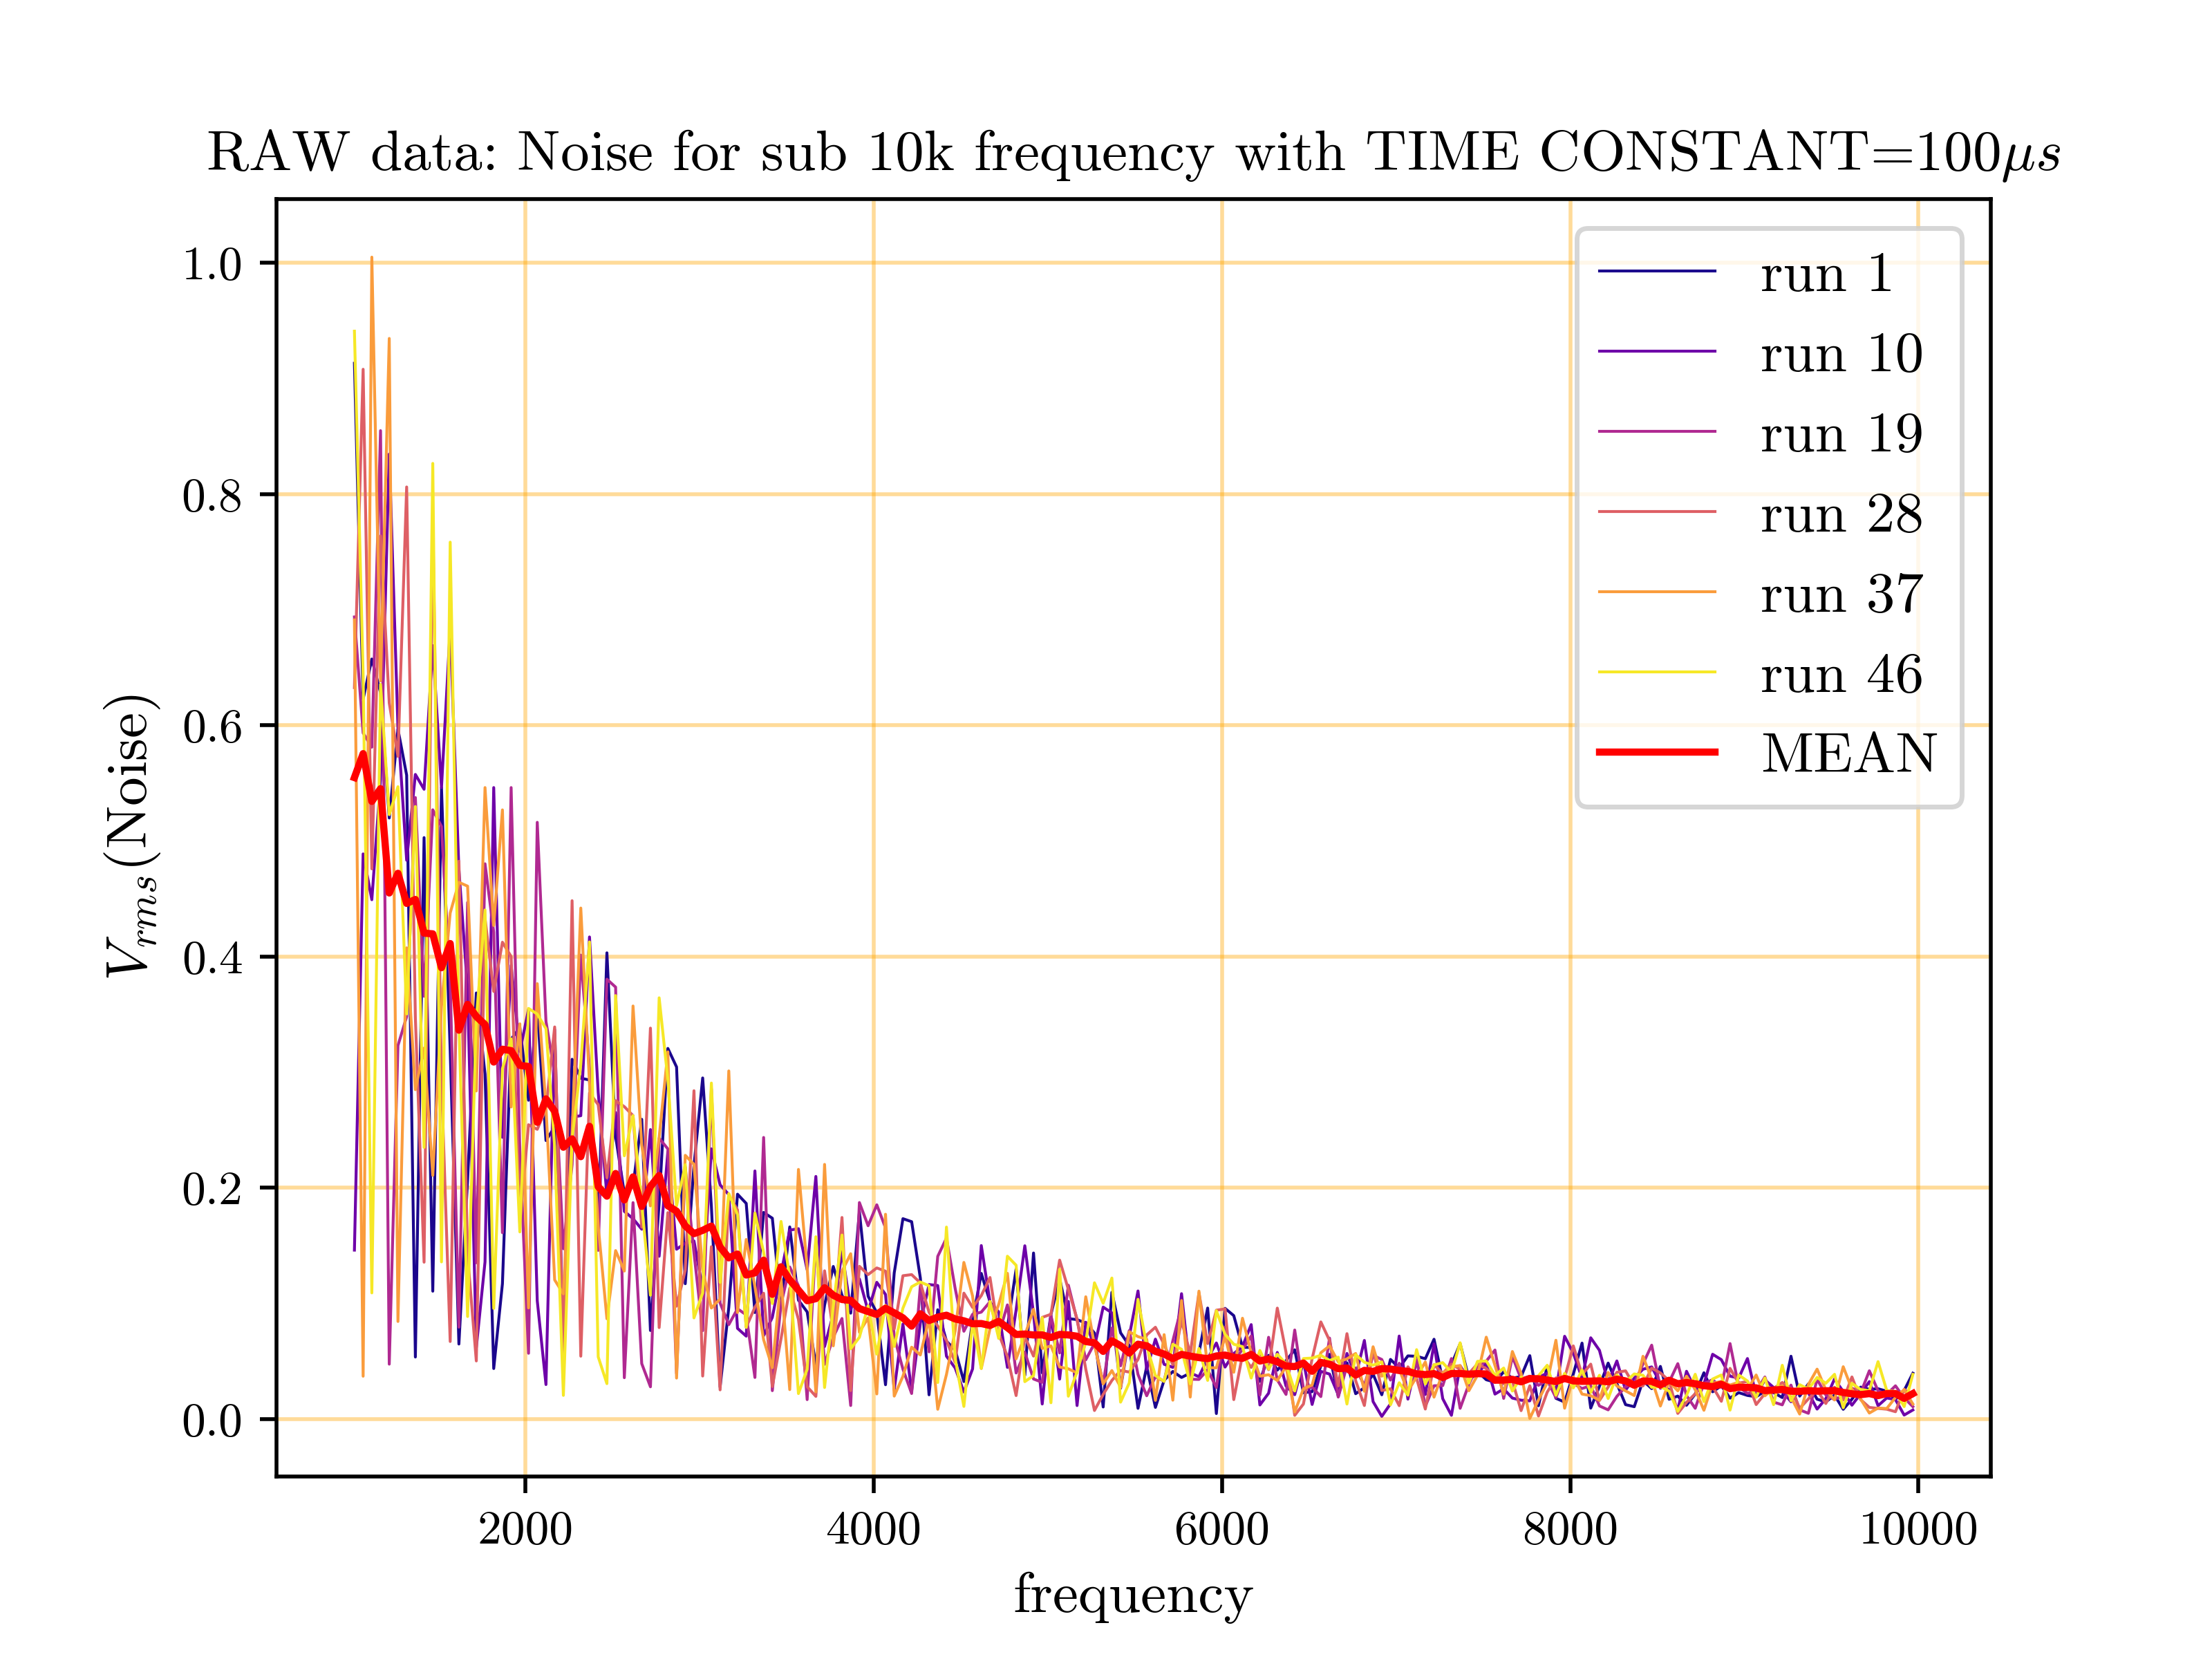
\includegraphics[width=.5\textwidth,trim={.5cm 0cm 1cm 0cm}, clip]{raw_1000_100us.png}}
\caption{This is row data for 1k to 10k frequency band TIME CONSTANT = $100\mu s$ and $12dB/oct$}
\end{figure}\\

Here initial results were quite random, which means we have to filter our data a bit. For this reason we used a basic filtering method. In this method the data are sorted out as minimum deviation from their minimum then we took the upper 5 to 10 results and took the mean of it. The basic implementation is as following,

Let, $X(f)$ as data point for specific $f$ and $Y(f)$ be sorted data with $n$ number of results,
\begin{align*}
\langle X(f) \rangle & = \sum_{i=0}^{N-1} X^{(i)}(f)\\
Y_n(f) & = min(t\: such\: that\: \# \{ s =\\
&   \lvert X(f)- \langle X(f)\rangle \rvert \;| s \geq t \} =n)\\
\langle Y(f) \rangle & = \sum_{i=0}^{n} Y^{(i)}(f)
\end{align*}

This is how we implemented it with python. If you wanna checkout whole code then it is in the appendix.

\begin{minted}[%
breaklines,    
breakanywhere,
mathescape,
xleftmargin=20pt,
linenos]{python}
for datapoint in data:
    count+=1
    if datapoint[0]==index:
        temp_erray.append(float(datapoint[1]))
    else:
        nlist = array(temp_erray,dtype=float)
        m = mean(nlist)
        sorted_deviation = argsort(abs(nlist - m))
        filtered_nlist = nlist[sorted_deviation[:points]]
        indexonelist = array([index]*points)
        final_list= column_stack((indexonelist,filtered_nlist))

\end{minted}

Also, as discussed from the previous section we have to correct these terms with ENBW. Time constant (T)= 100$\mus$ and roll-off =12 $dB/oct$
       
\[
ENBW = \frac{1}{8T} = 1250 Hz 
\]



\begin{figure}[hbt!]
\centering{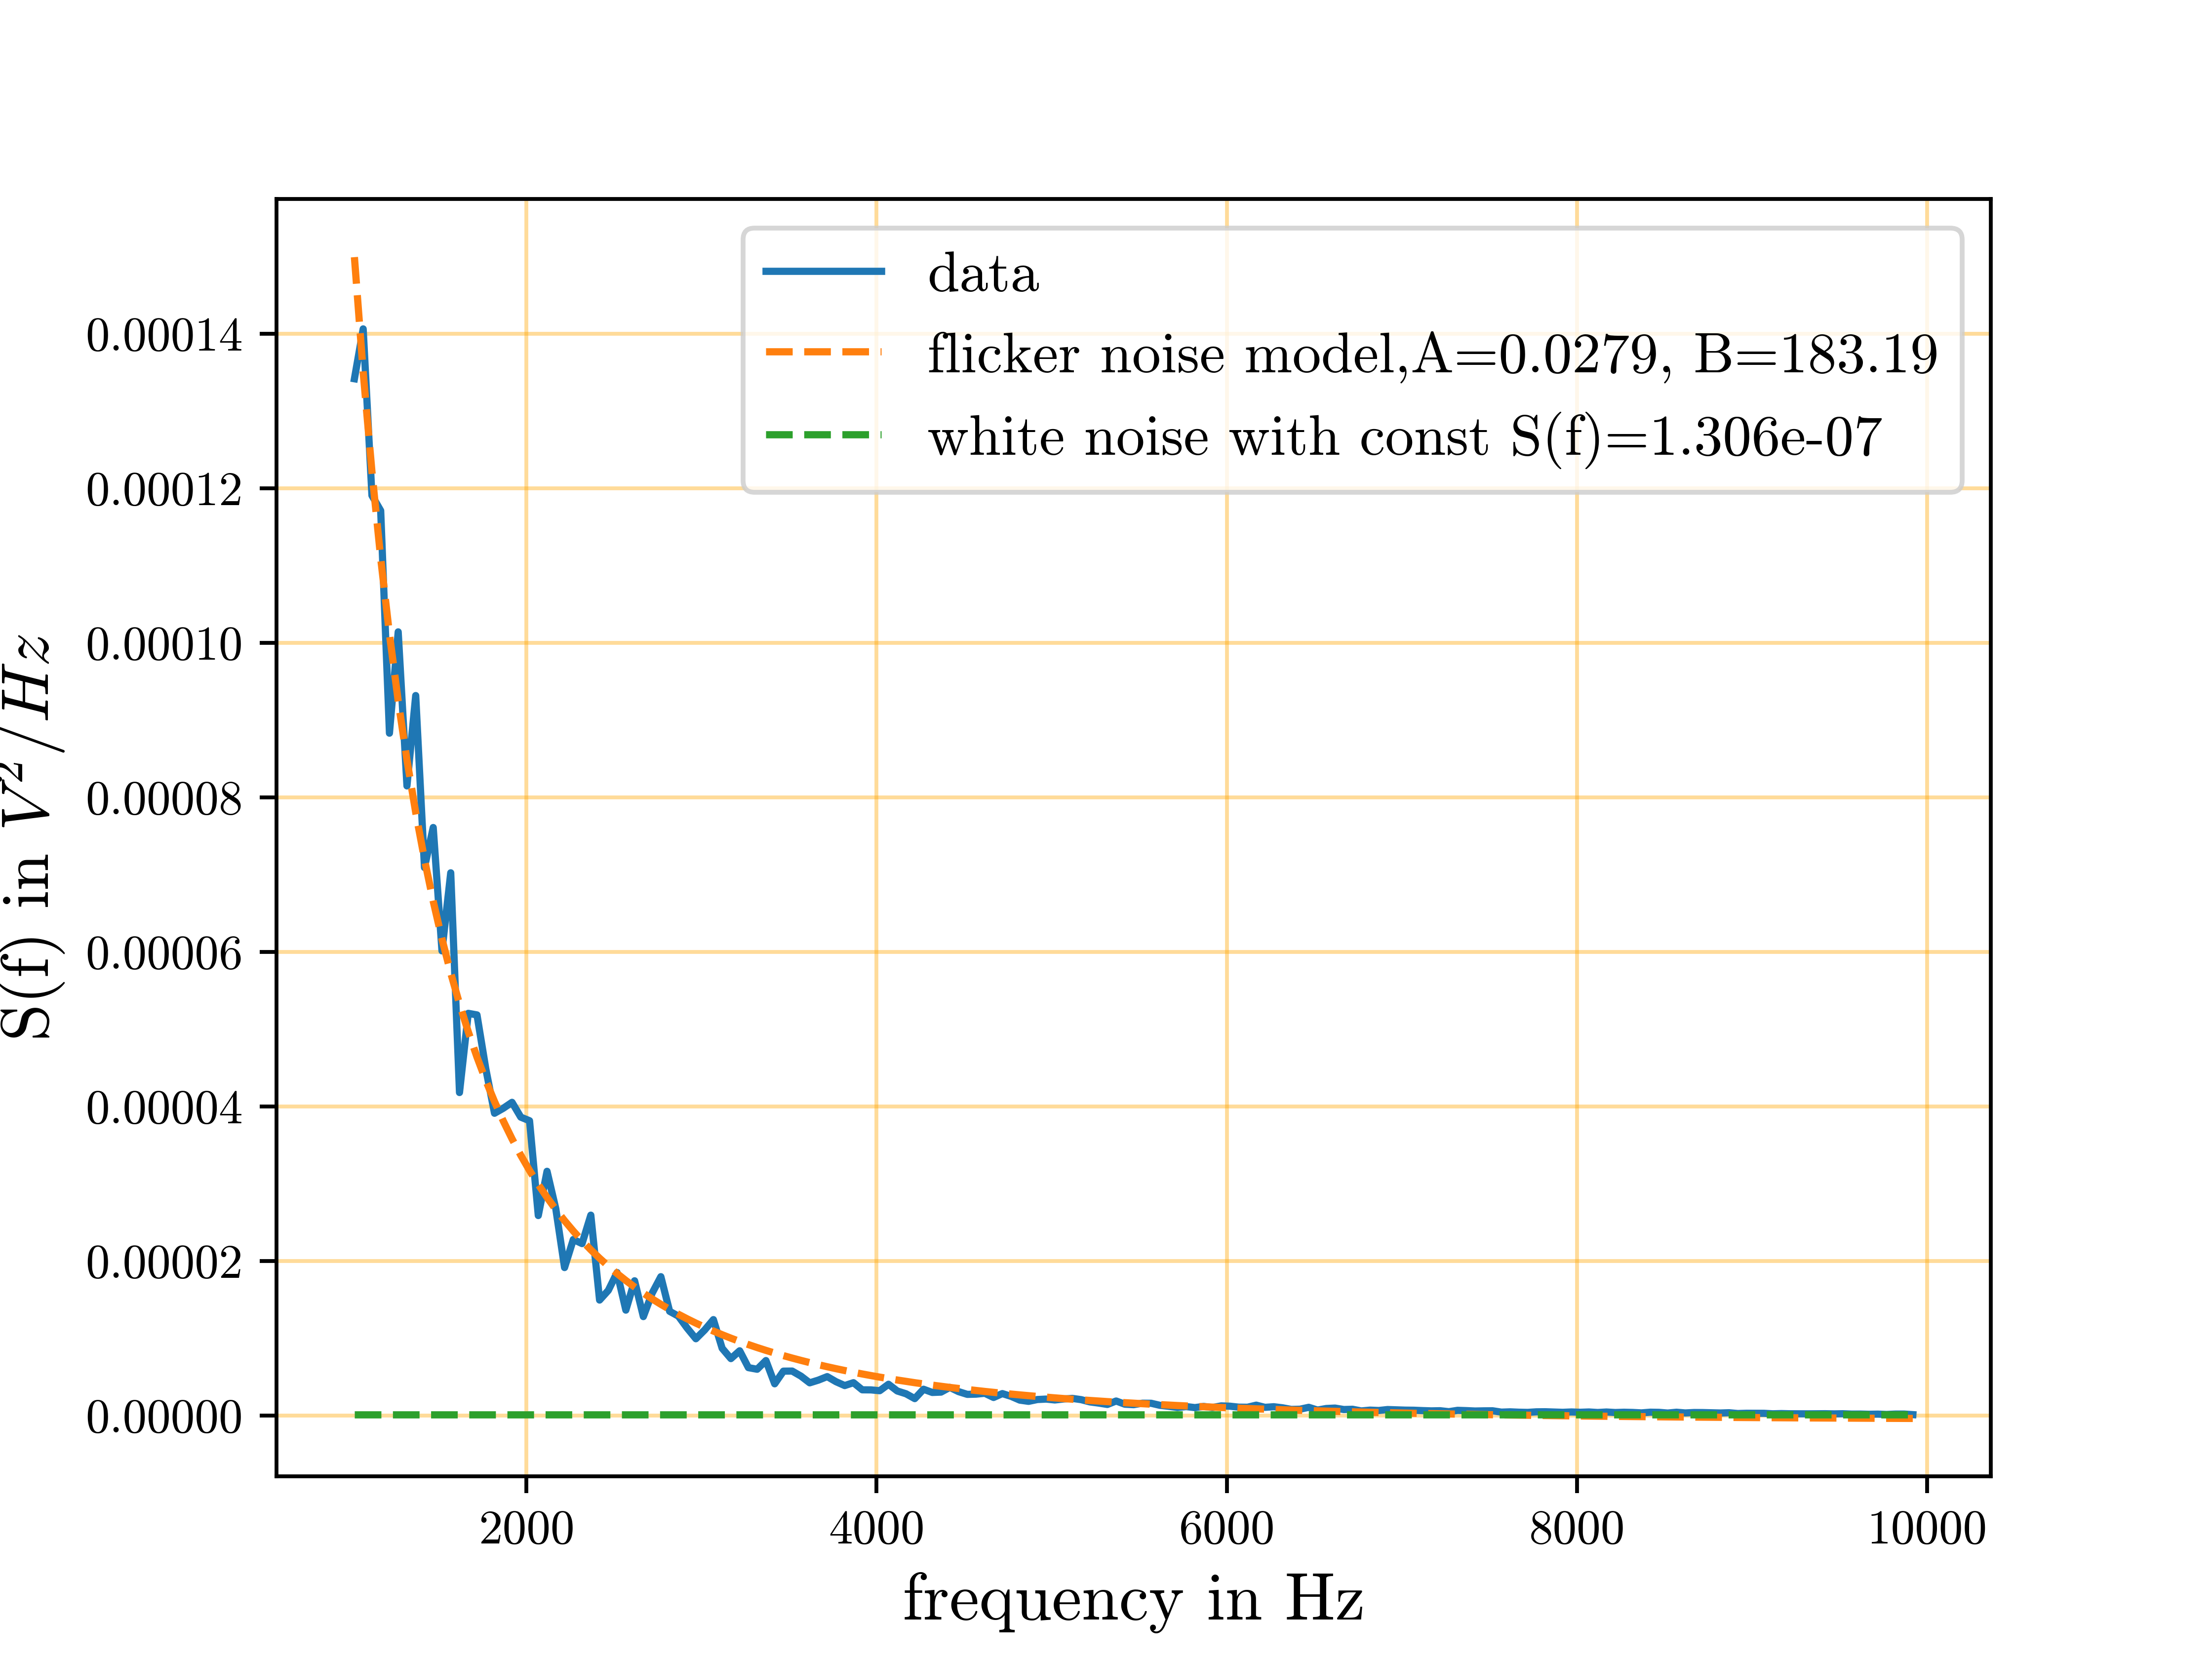
\includegraphics[width=.5\textwidth]{final_1000_100us.png}}
\caption{final analysed data for 1k to 10k hertz frequency with TIME CONSTANT = $100\mu s$ and $12dB/oct$}
\end{figure}\\
 
Here we can see some traces of flicker noise. Parameterized as follows,


\begin{align*}
S(f) & = \frac{\gamma}{f^{\alpha}}
\end{align*}

Here, $\gamma$ and $\alpha$ determine the nature of flicker noise. Results are from theoritical section.

\begin{align}\label{eq1}
S_{flicker}(f) & = 5.90923491 \frac{1}{f^{1.34677368}}\\
S_{white}(f) & =2.0644381e-05
\end{align}


\subsection{Very low frequency: upto 1 hertz}

Let's take a second data set where we have sub hertz frequency data. This data set have each frequency with corresponding 50 values. Raw data looks like figure \ref{rawsubhz}.


\begin{figure}[hbt!]
\centering{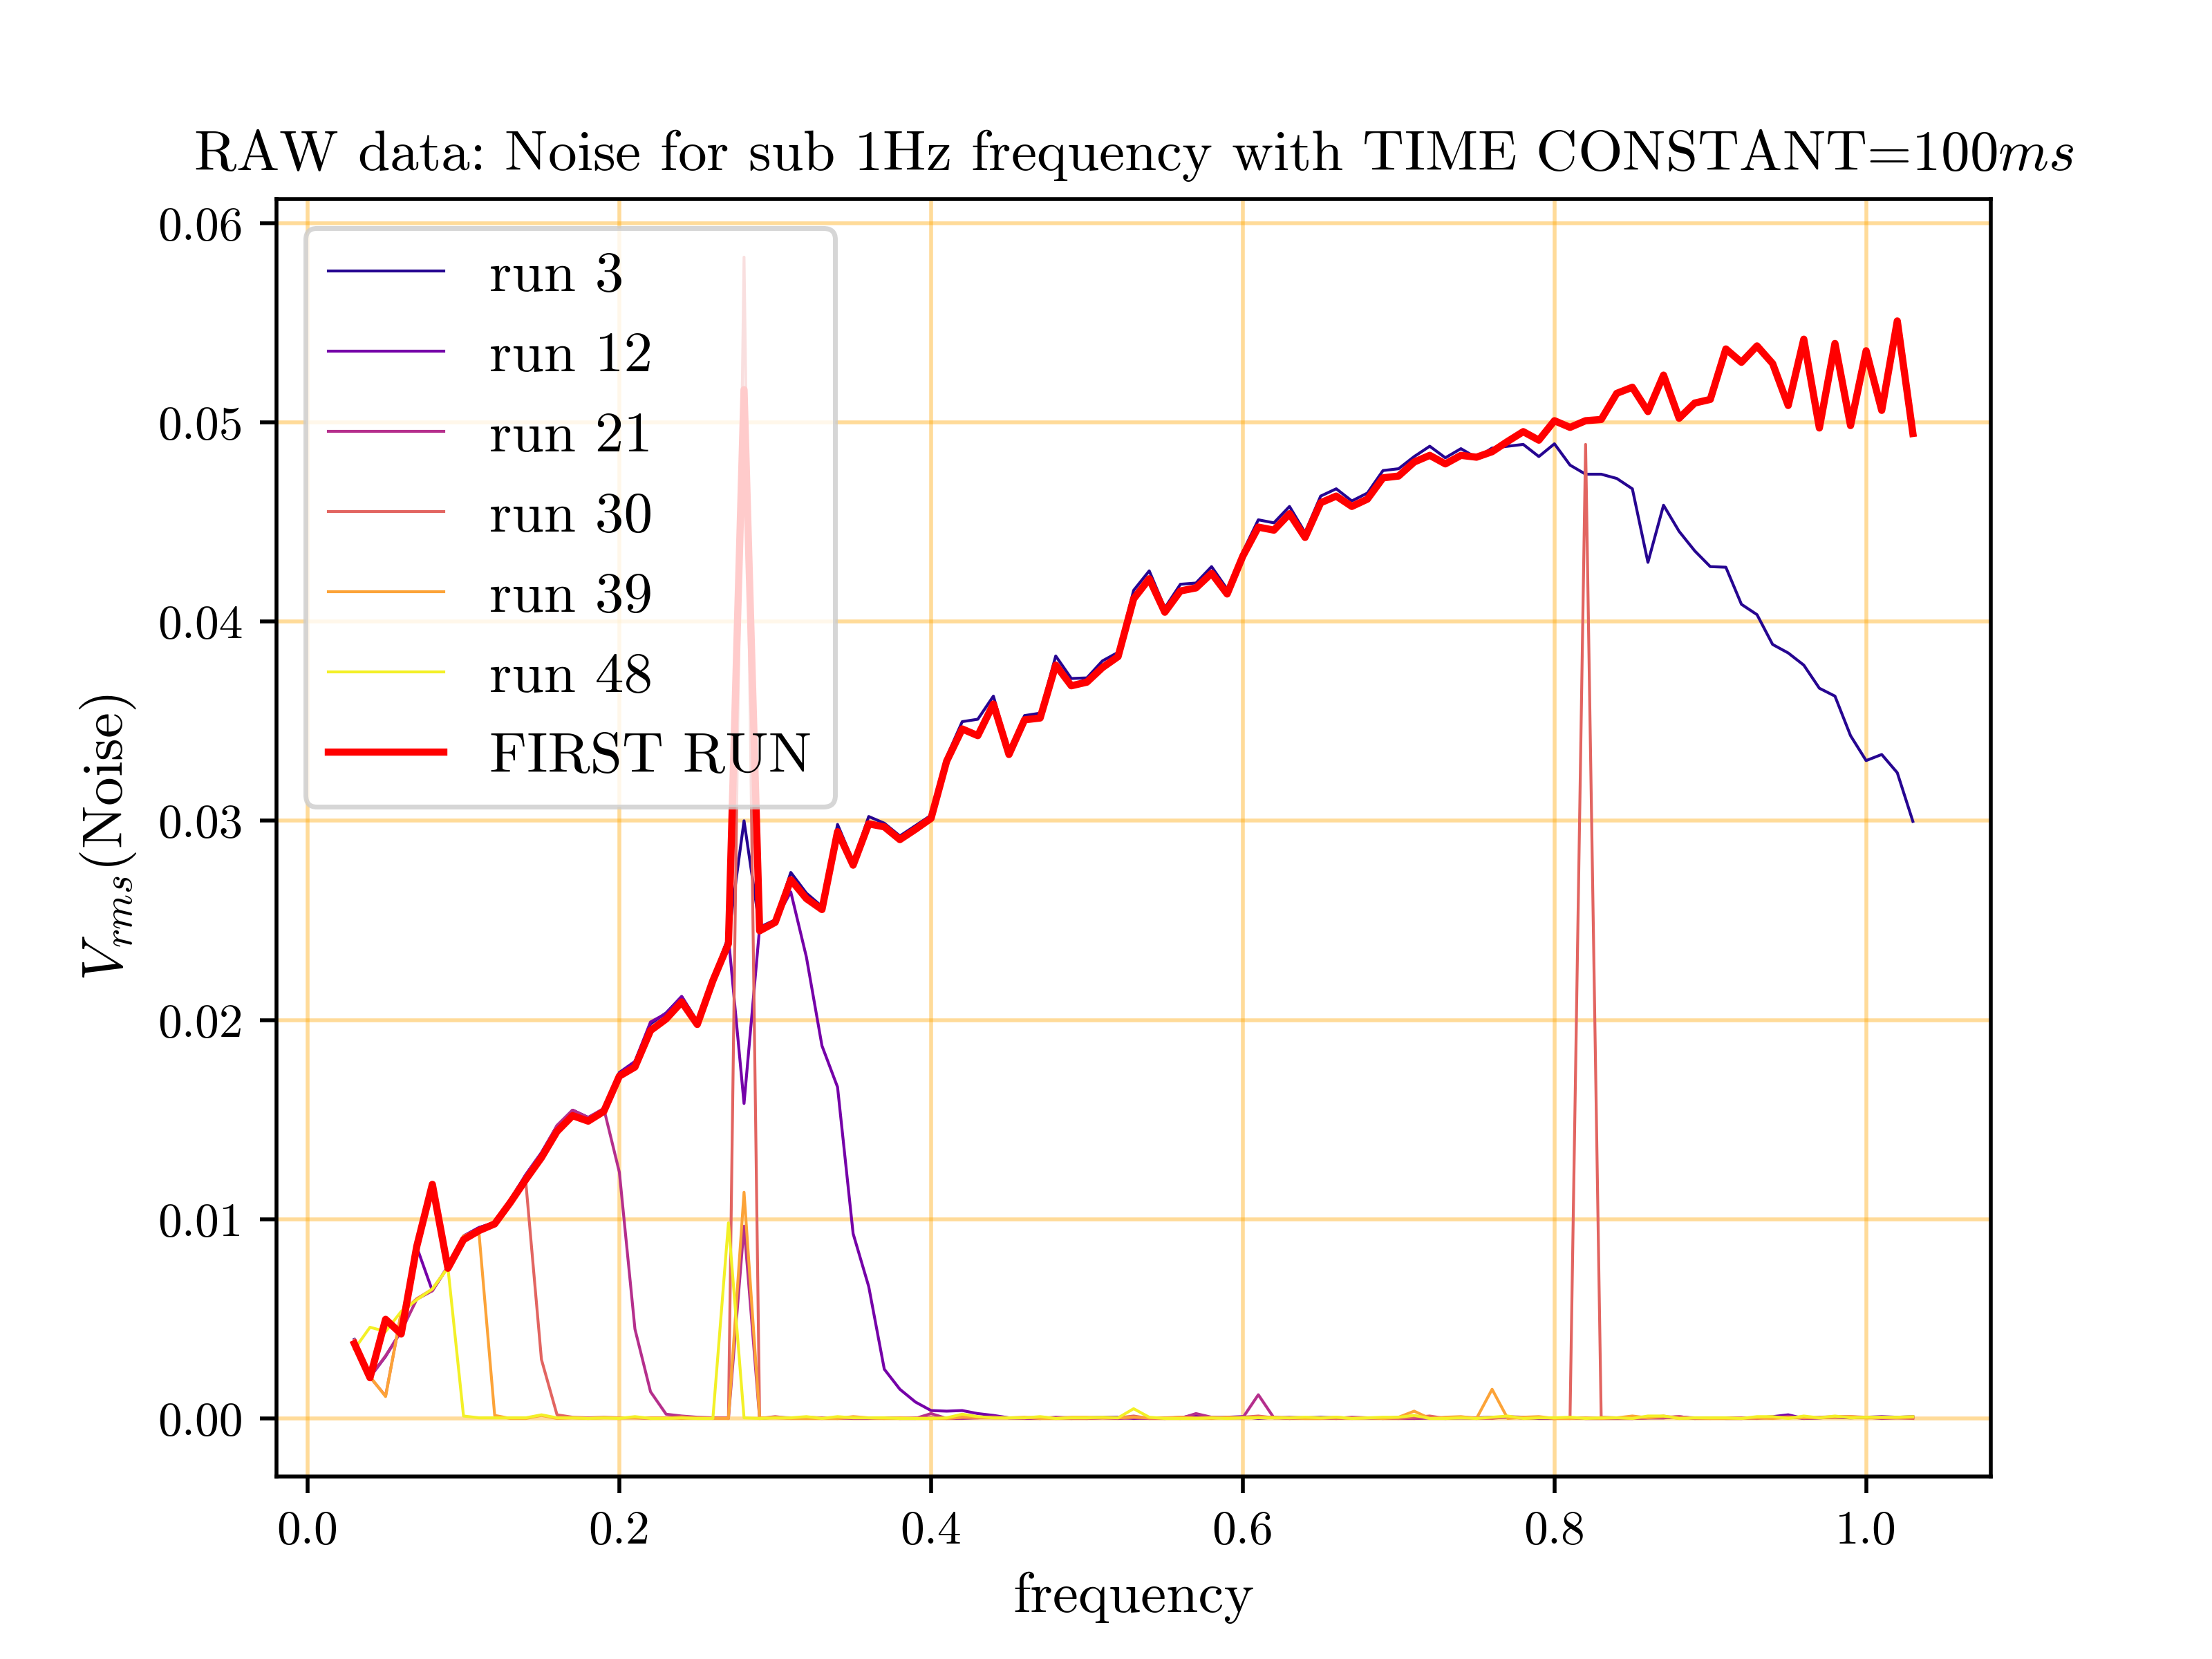
\includegraphics[width=.5\textwidth]{raw_1_100us.png}}
\caption{This is row data for sub one hertz band with TIME CONSTANT = $100ms$ and roll of factor $12dB/oct$} 
\label{rawsubhz}
\end{figure}\\


For analysing data ENBW is calculated for TIME CONSTANT = $100ms$ and roll of factor $12dB/oct$},

       
\[
ENBW = \frac{1}{8T} = 1.25 Hz 
\]

Final data will be look like this,

\begin{figure}[hbt!]
\centering{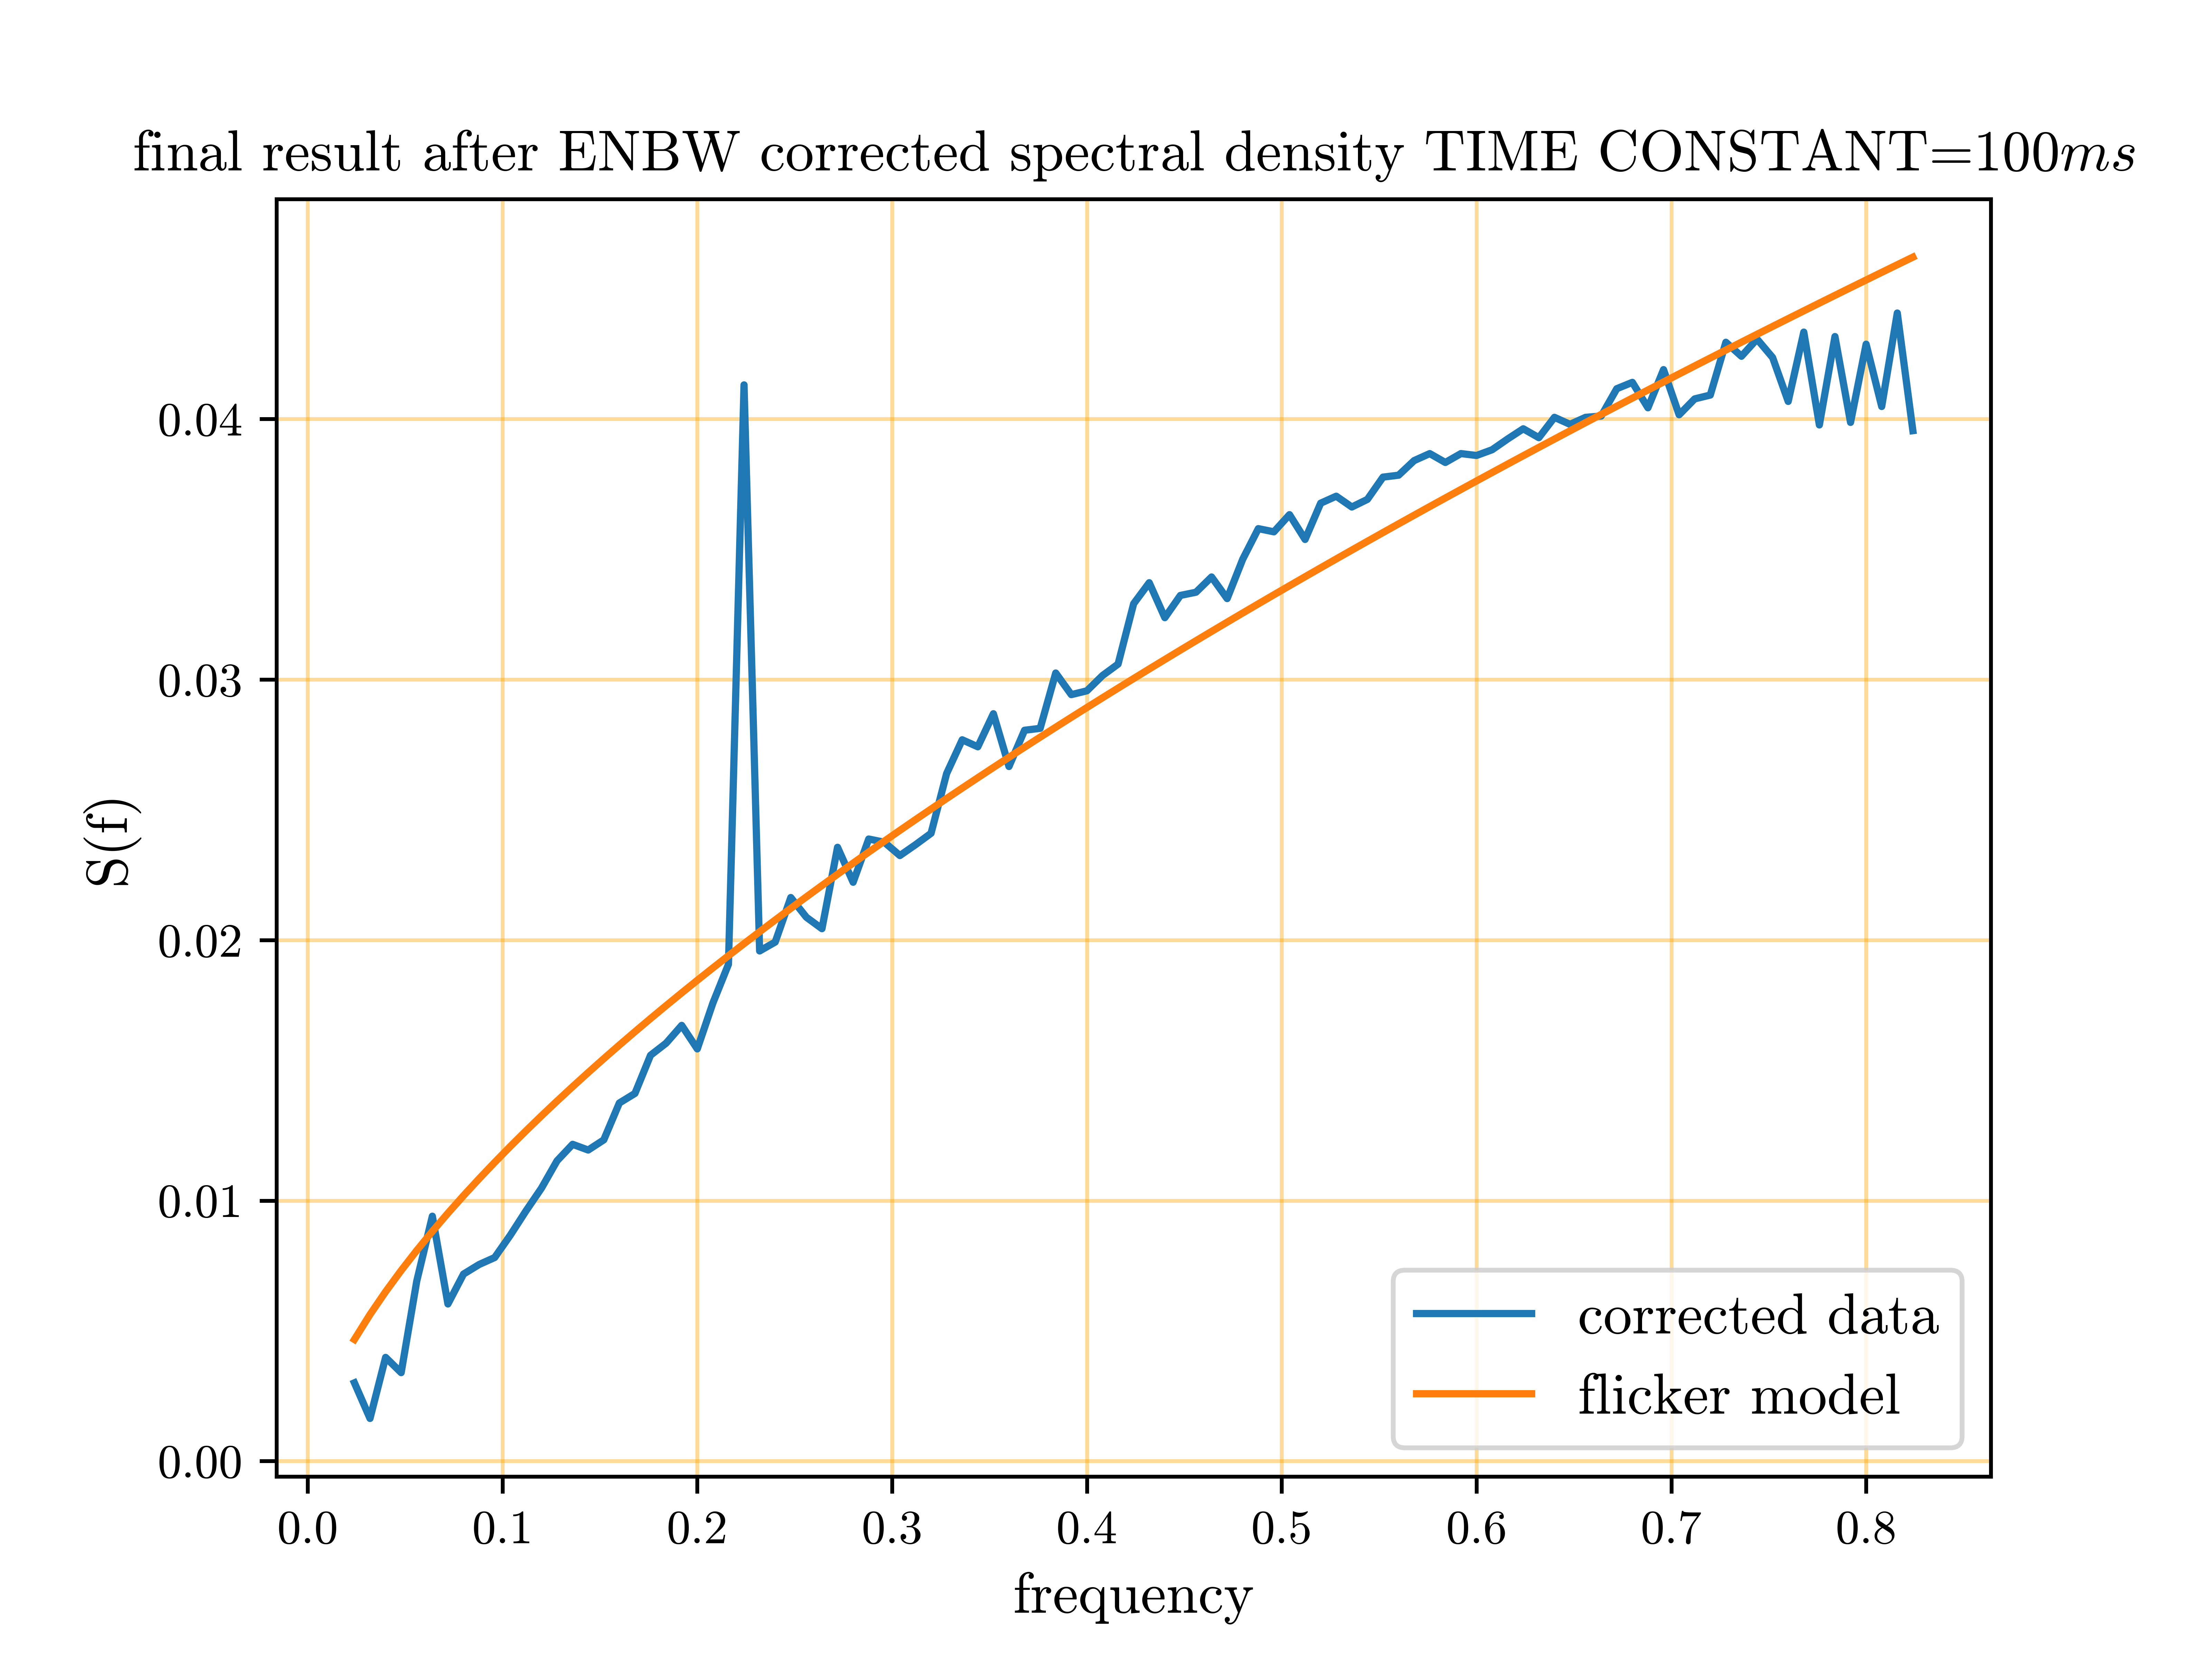
\includegraphics[width=.5\textwidth]{final_1_100ms.png}}
\caption{final analysed data for sub one hertz band with TIME CONSTANT = $100ms$ and roll of factor $12dB/oct$}
\end{figure}\\


Here data feeted at negative $-alpha$,

\begin{align}\label{eq2}
S_{flicker}(f) & =  \frac{-0.64836618}{f^{-0.64836618}}
\end{align}

Here two things is important $\alpha < 0$ and $\gamma$ is small.

\subsection{High frequency data: up to 100k hertz}

Same as we discussed previously raw data is given here, we have up to 50khz frequency domaoin data,


\begin{figure}[hbt!]
\centering{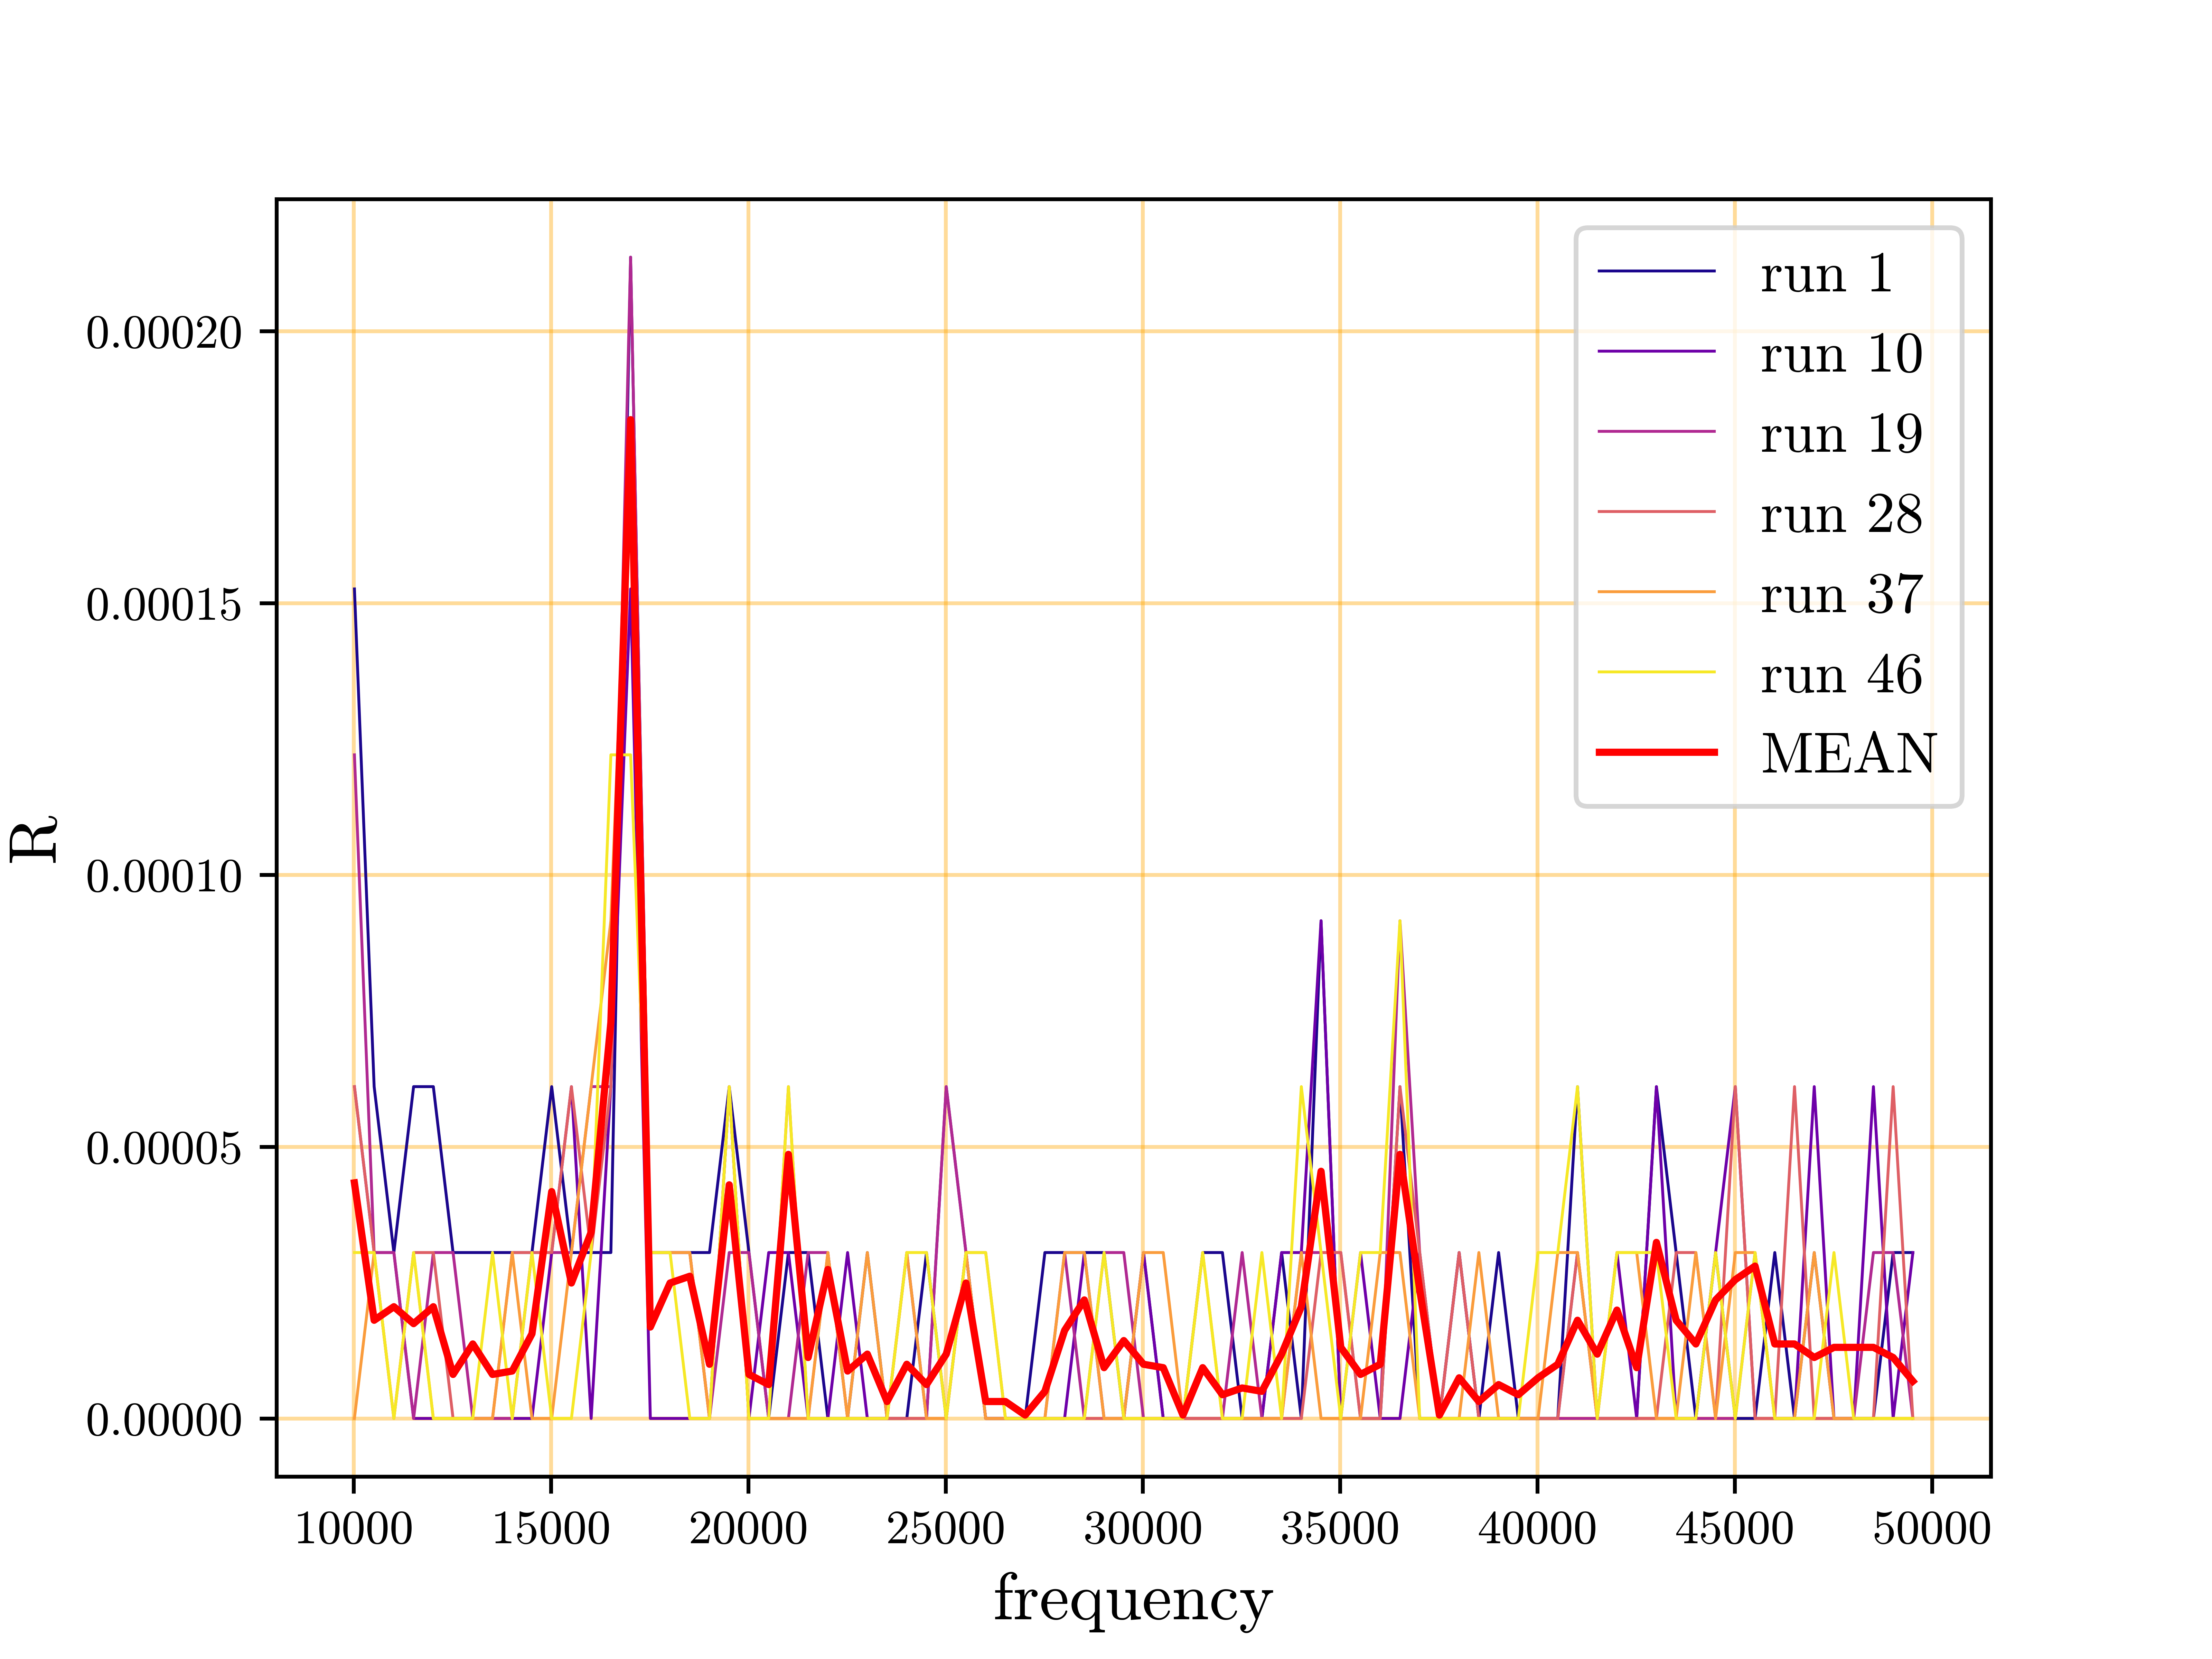
\includegraphics[width=.5\textwidth]{raw10000100ms.png}}
\caption{This is row data for high frequency band with TIME CONSTANT = $100ms$ and roll of factor $12dB/oct$} 
\label{raw100k}
\end{figure}\\

same as previous sections, we sorted data and take ENBW calculations at here.

\begin{figure}[hbt!]
\centering{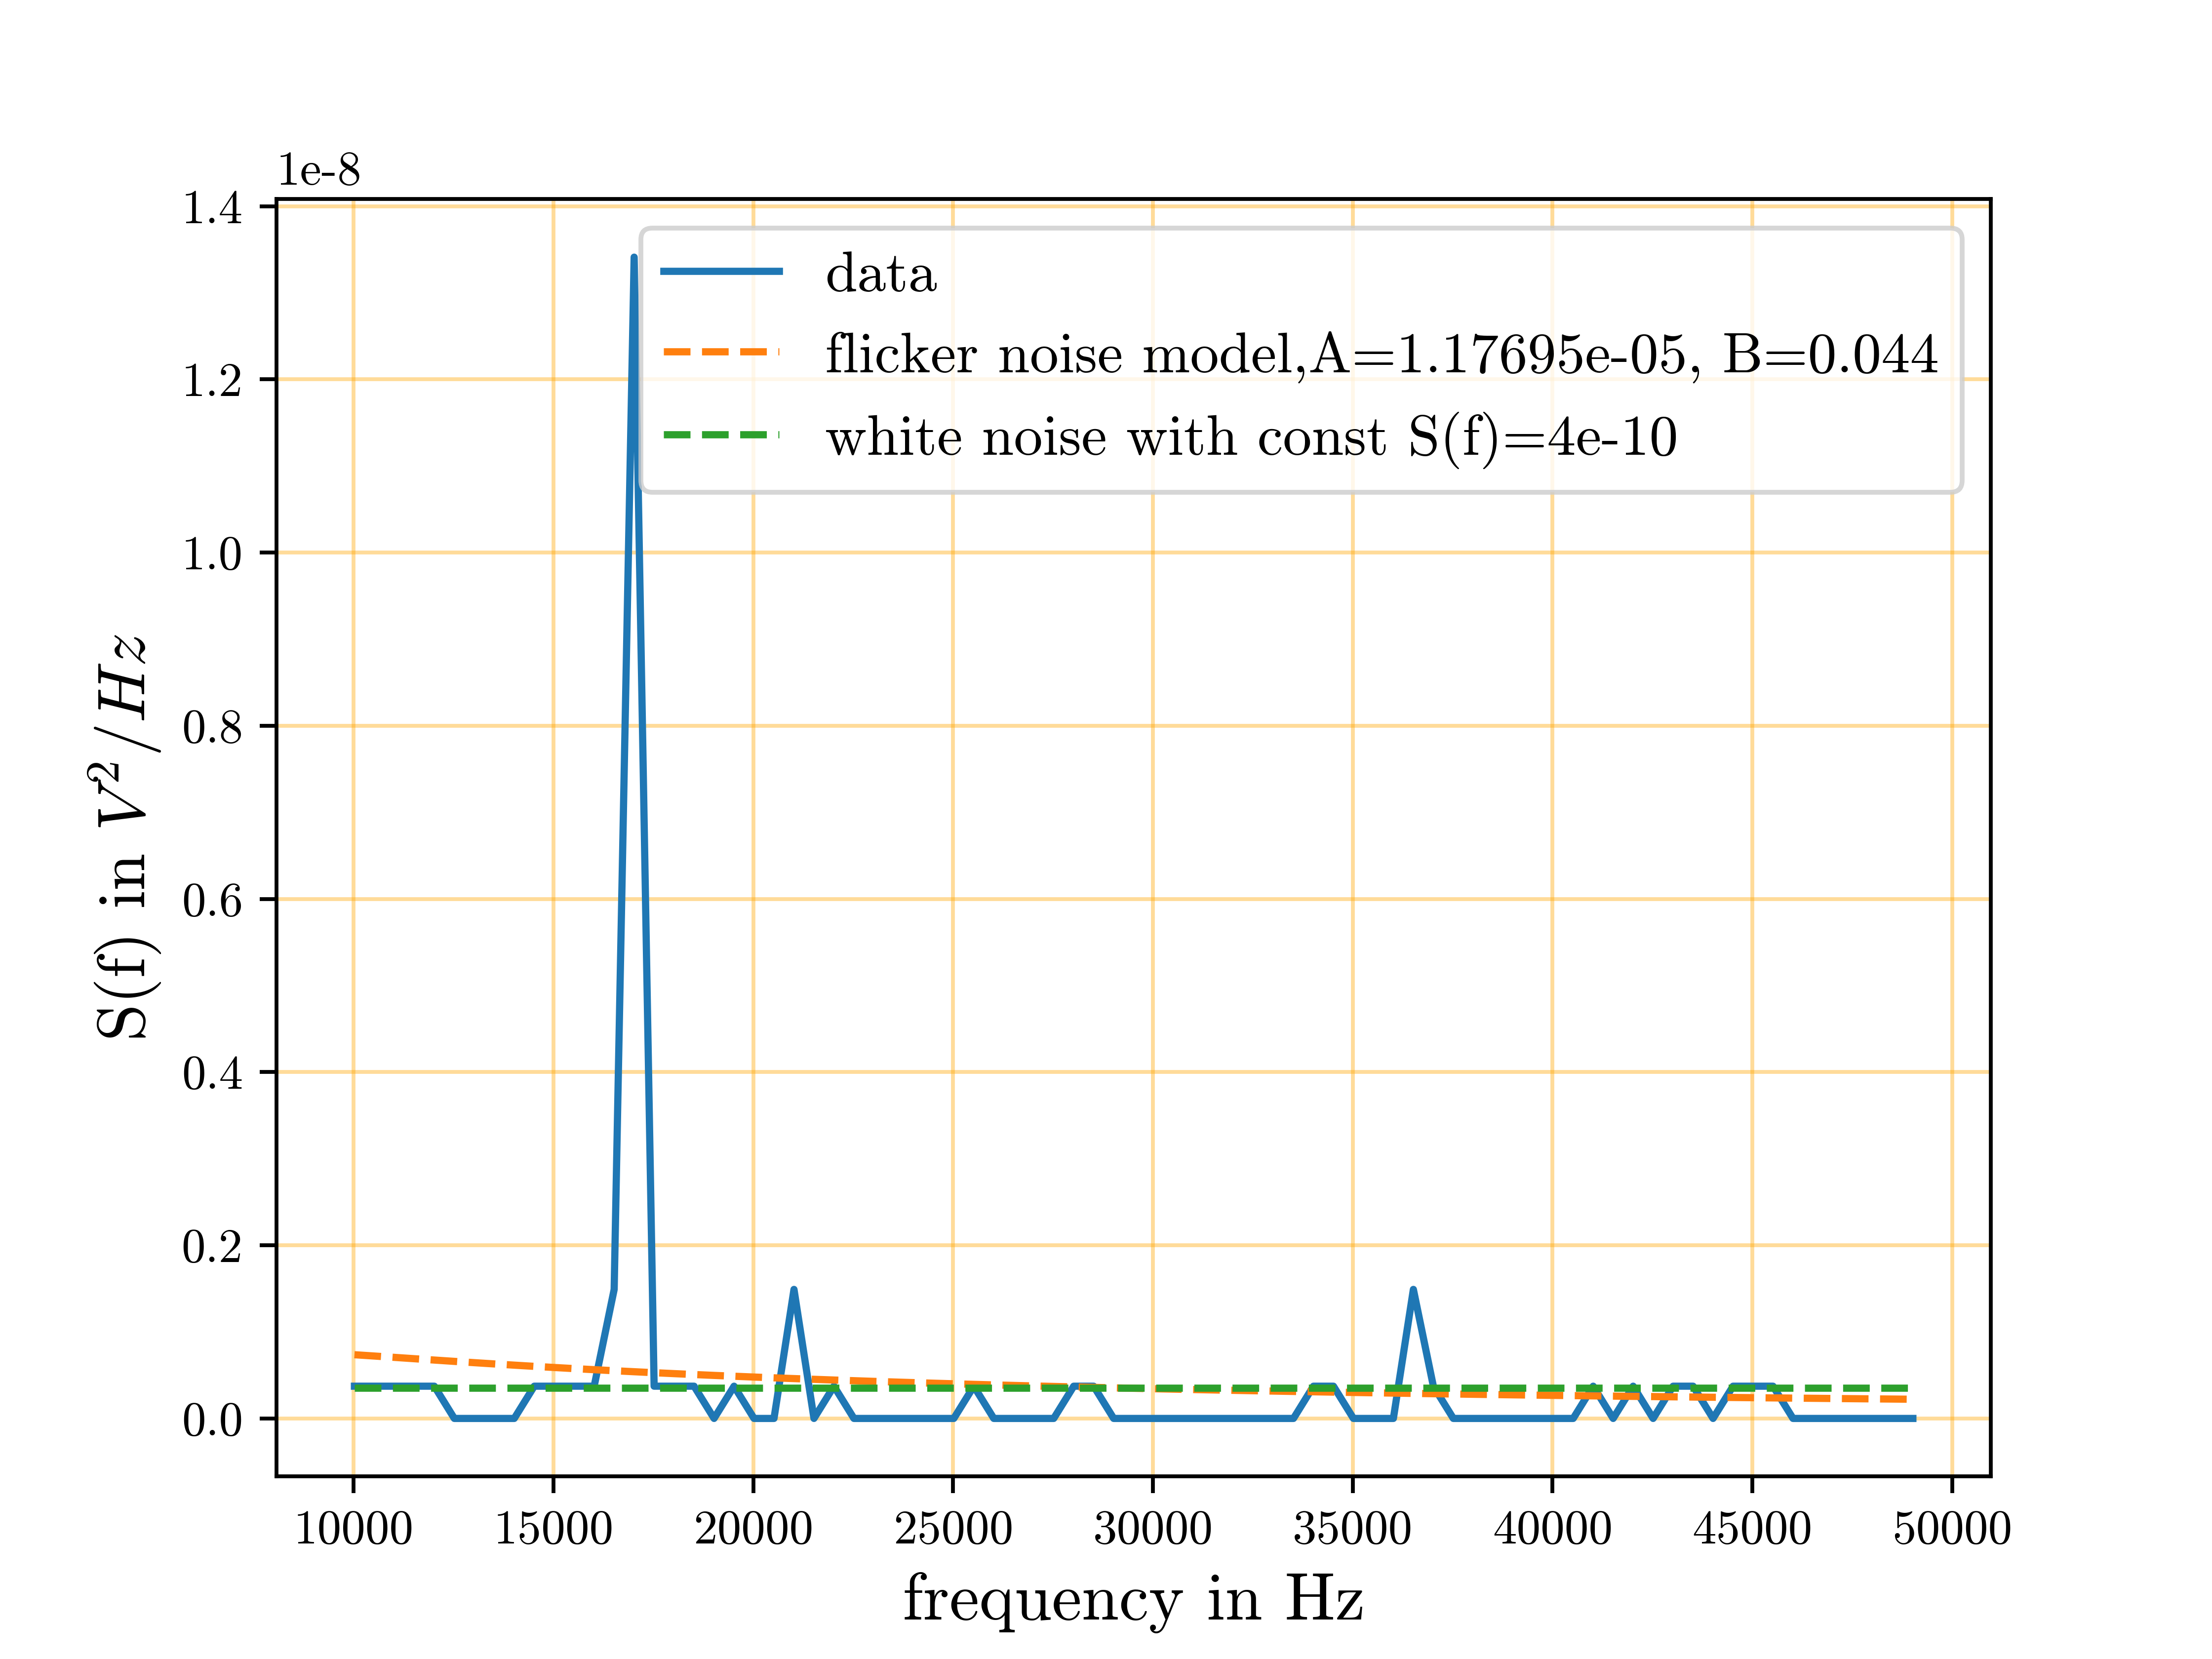
\includegraphics[width=.5\textwidth]{final_10000_100ms.png}}
\caption{final analysed data for high frequency band with TIME CONSTANT = $100ms$ and roll of factor $12dB/oct$}
\end{figure}\\

the noise spectral density is as following.

\begin{align}\label{eq3}
S_{flicker}(f) & = \frac{0.13707877}{f^{0.92287006}}\\
S_{white}(f) & = 1.20525914e-05
\end{align}


Here this parameters are similar to that of first data set aka low frequency data.
